\begin{frame}{Ice People Family Tree}
    \note{\scriptsize
    \begin{itemize}

        \item Diving into the narrative intricacies of the 47-book saga,
        we're brought face-to-face with a sprawling family tree that traces its lineage
        back to the matriarch Silja Arngrímsdóttir and her cursed beau, Þengill the good.

        \item Their descendants' tangled relationships are laid out here,
        and it's impossible to ignore the density of the connections --
        hinting at a significant amount of inbreeding.
        This compact lineage, while perhaps challenging for readers (and narrators!)
        to digest given its incestuous undertones, does offer us a silver lining --
        it's surprisingly \emph{slide-friendly}. Managing to represent 17 generations in one visual
        would generally be a challenge, but this is a rare exception.

        \item Cursed family members are color-coded: yellow for \emph{virtuous}, green for \emph{malevolent}, and pink for those who found \emph{redemption}.

        \item As we scan through the tree, it's curious to note that the distribution of the curse
        doesn't seem to follow a strict genetic pattern. Entire generations sometimes escape its grasp,
        suggesting that Margit perhaps allowed a degree of creative freedom over genetic accuracy in
        deciding who bears the curse.

        \item This intricate web of relationships, filled with cursed figures,
        highlights the need for a data-driven approach to unravel and understand Margit's artistic choices.
        \end{itemize}
}
    \centering
    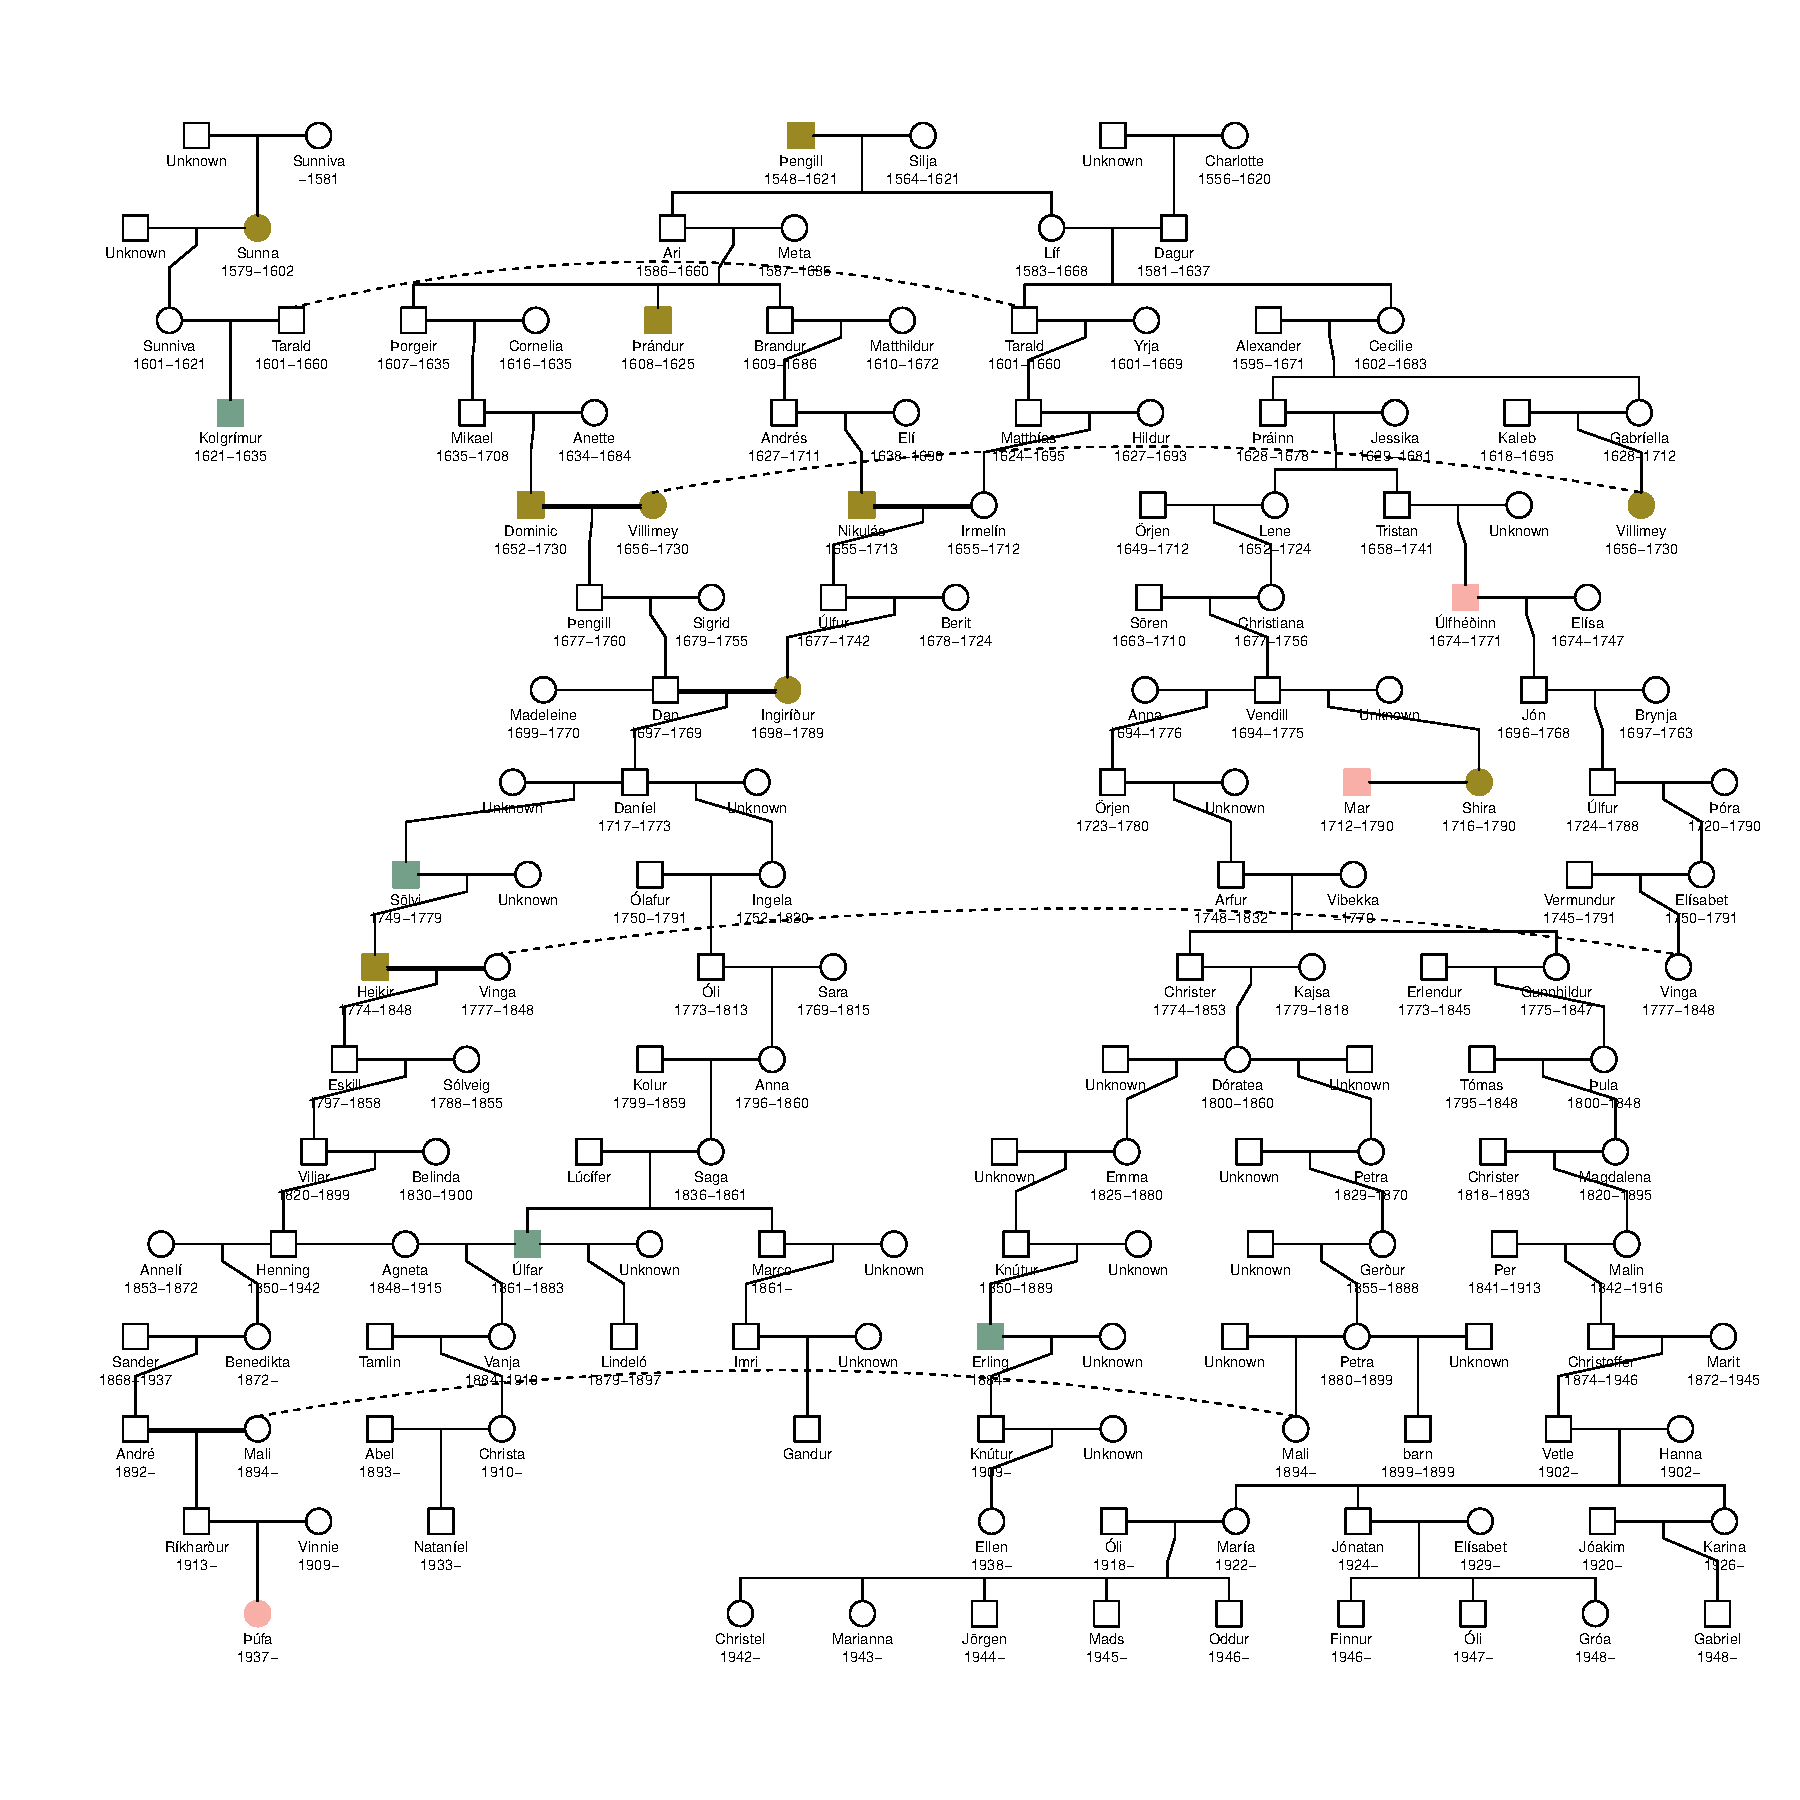
\includegraphics[height=.9\textheight]{../rek-data-beers/R/figures/family_tree}
\end{frame}

\begin{frame}{Ice People Family Gantt Chart}
    \note{\scriptsize
    \begin{itemize}
        \item To decipher the complex family tree and its concurrent relationships,
        we turned to a \emph{data transformation}: the \emph{Gantt} chart,
        usually a tool for project timelines, but here, it's a brilliant
        visualization of lifespans and intersecting narratives.

        \item Spanning from the mid-1600s to the 1960s, this chart offers clear insights
        into overlapping lifetimes, painting a vivid picture of contemporaneous
        characters.

        \item Margit frequently intertwines character narratives,
        often through romantic unions. This attraction amongst cousins is
        both a narrative device and a manifestation of their shared, cursed lineage.
        Despite many generations, the family size stays around 20 members, peaking at 30 later on.

        \item Typically, 1-2 cursed individuals from the Ice People are alive at any given time. However, a spike occurs in the early 1700s with six simultaneous cursed beings.
        \item Mar, in particular, isn't directly of the Ice People. He's of the Taranqyes lineage, which traces back to their common ancestor the infamous Þengill the Bad.
        \item The gaps in the family tree regarding cursed individuals suggest that the Taranqyes lineage might be the ones carrying the curse for those missing generations, as the narrative asserts there's always one cursed person per generation.
        \end{itemize}
    }
    \centering
    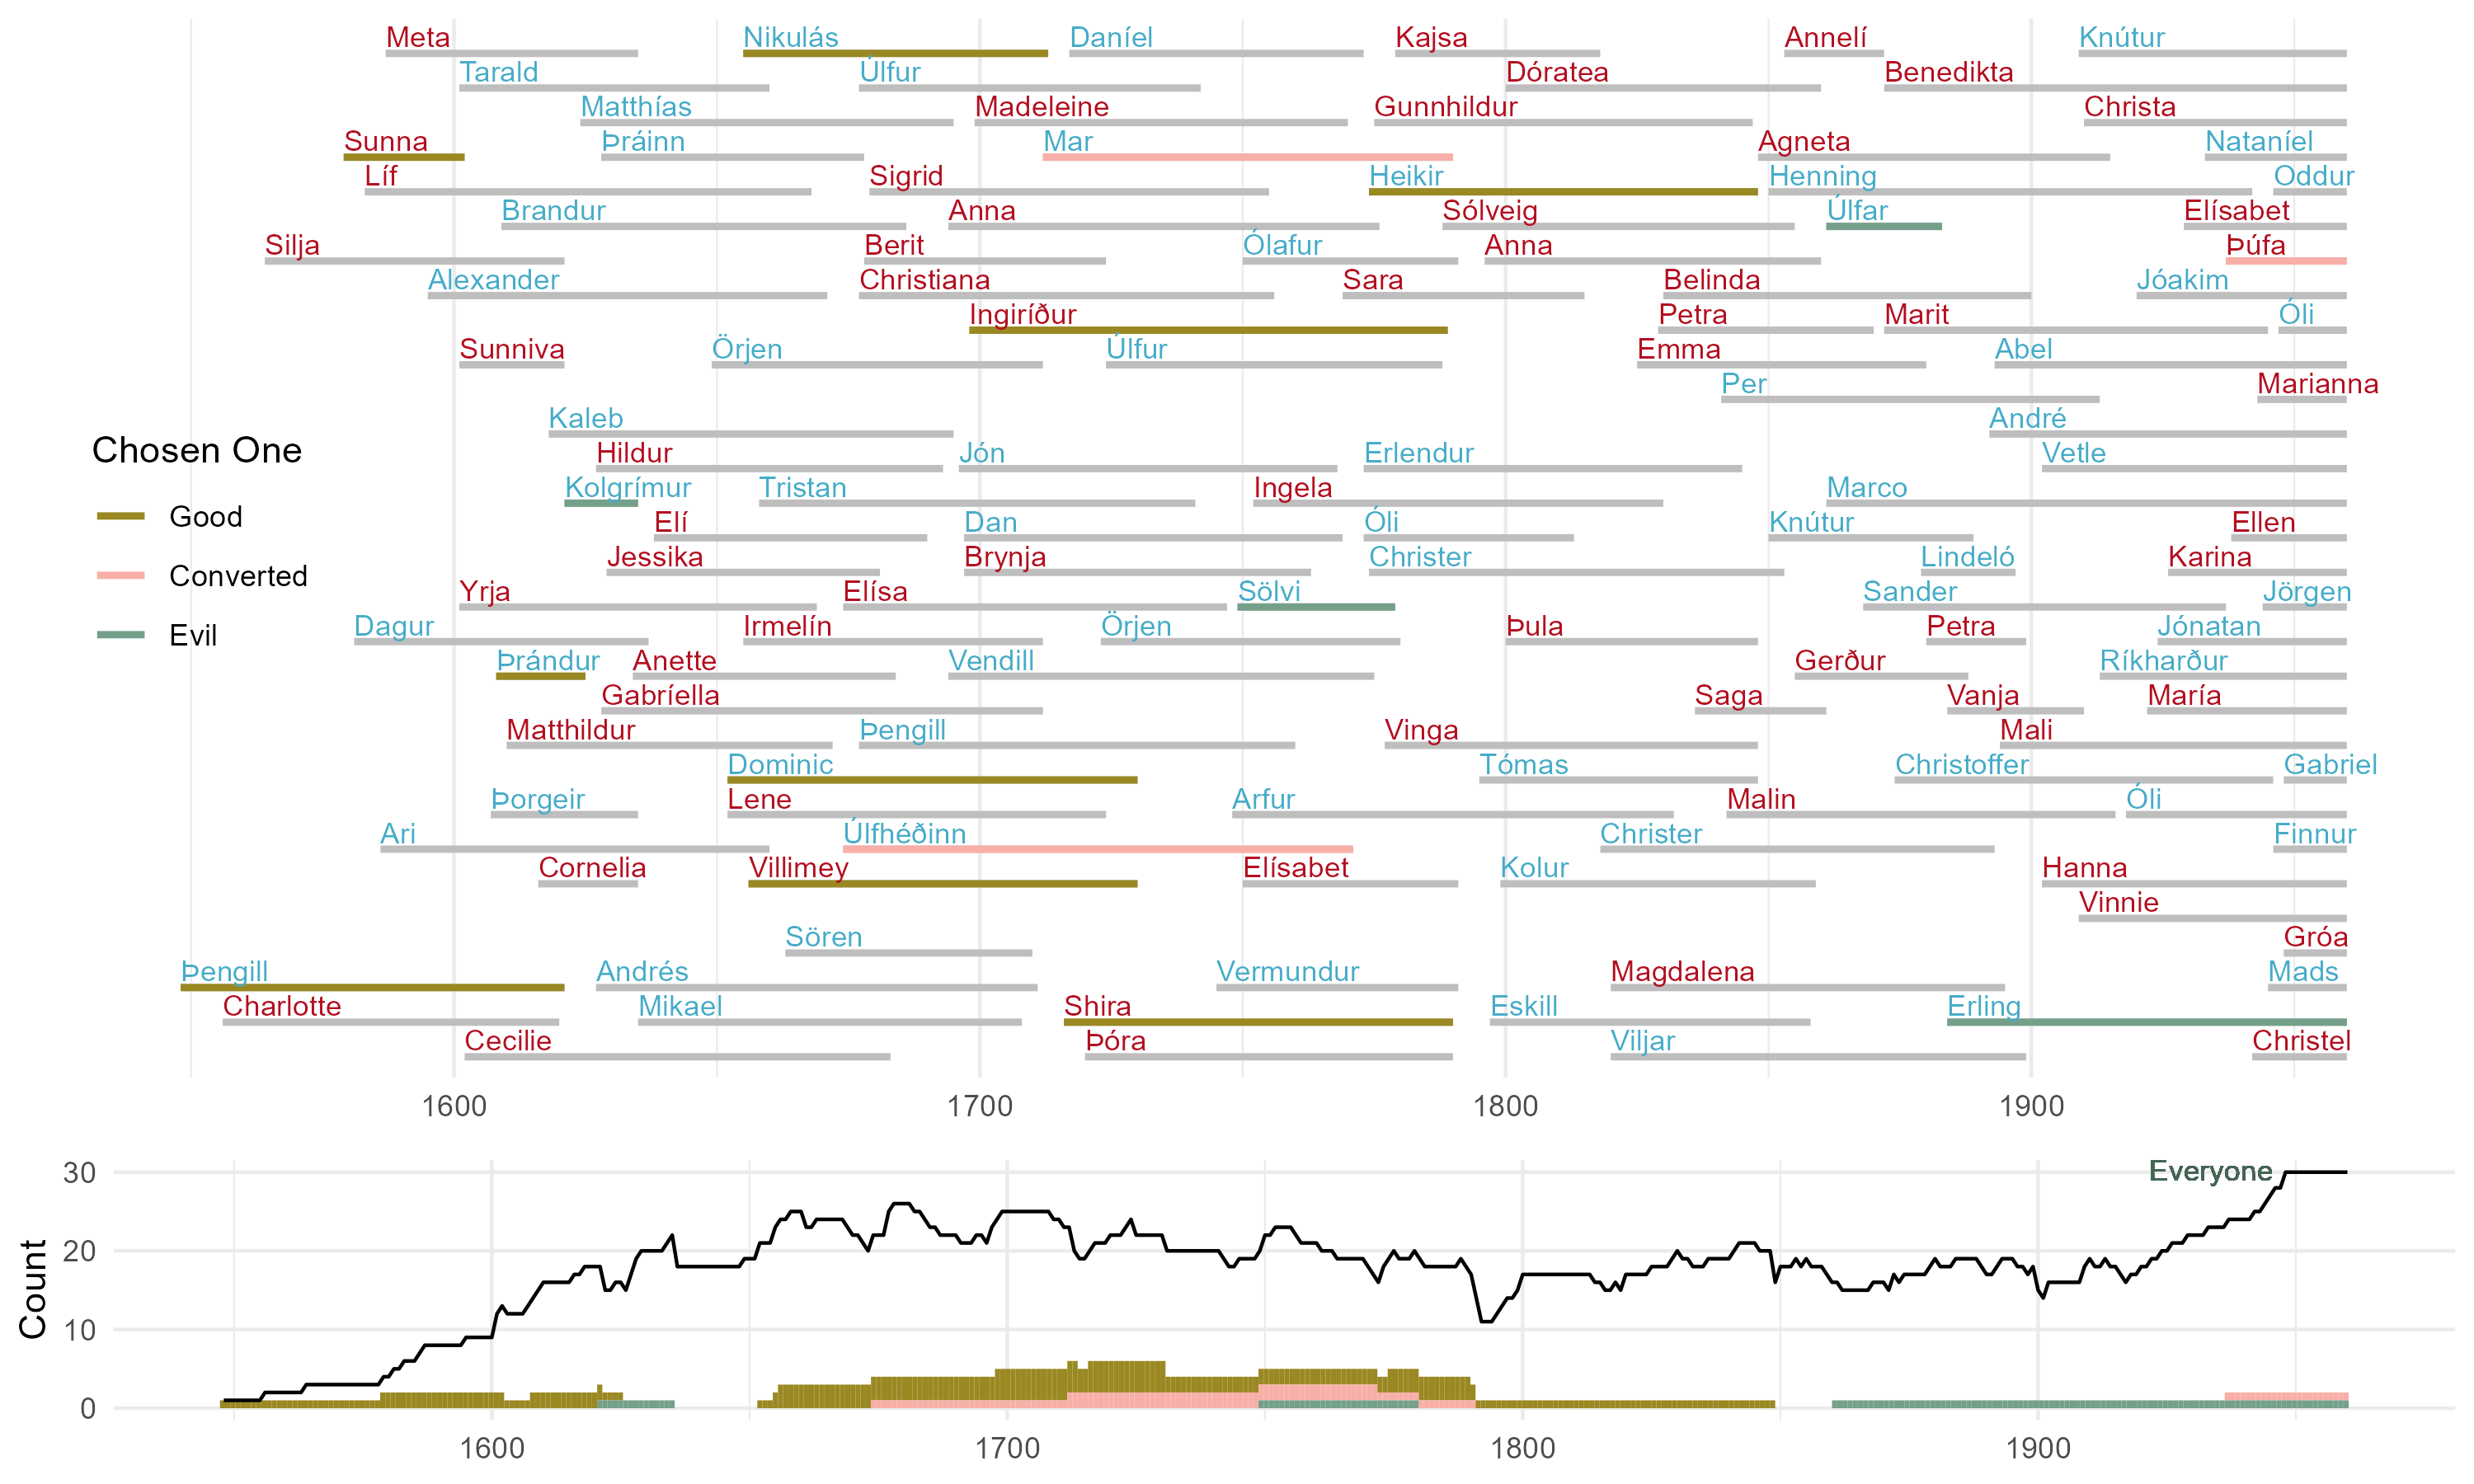
\includegraphics[width=\textwidth]{../rek-data-beers/R/figures/family_gantt}
\end{frame}

\begin{frame}{Lifespan of the Ice People}
\note{
\begin{itemize}
\item The data shows is a unique age \emph{bimodal distribution} diverging from the typical bell curve.
\item Many women, due to the curse, don't survive childbirth, leading to a life expectancy drop around the mid-20s.
\item Those women who overcome this hurdle often live up to 70 years, resulting in a second age peak.
\item Margit ensures symmetry: while women face childbirth peril, men, characterized by their recklessness, confront their own early-life dangers. Those men who navigate past these threats also enjoy an extended lifespan, reinforcing the bimodal pattern.
\item Looking at relationships:
 A third of characters are unrelated to the Ice People – or \emph{muggles}.
 Half are pure-bloods, having both parents from the Ice People.
 The rest, about 15\%, are half-bloods.
\end{itemize}
}

    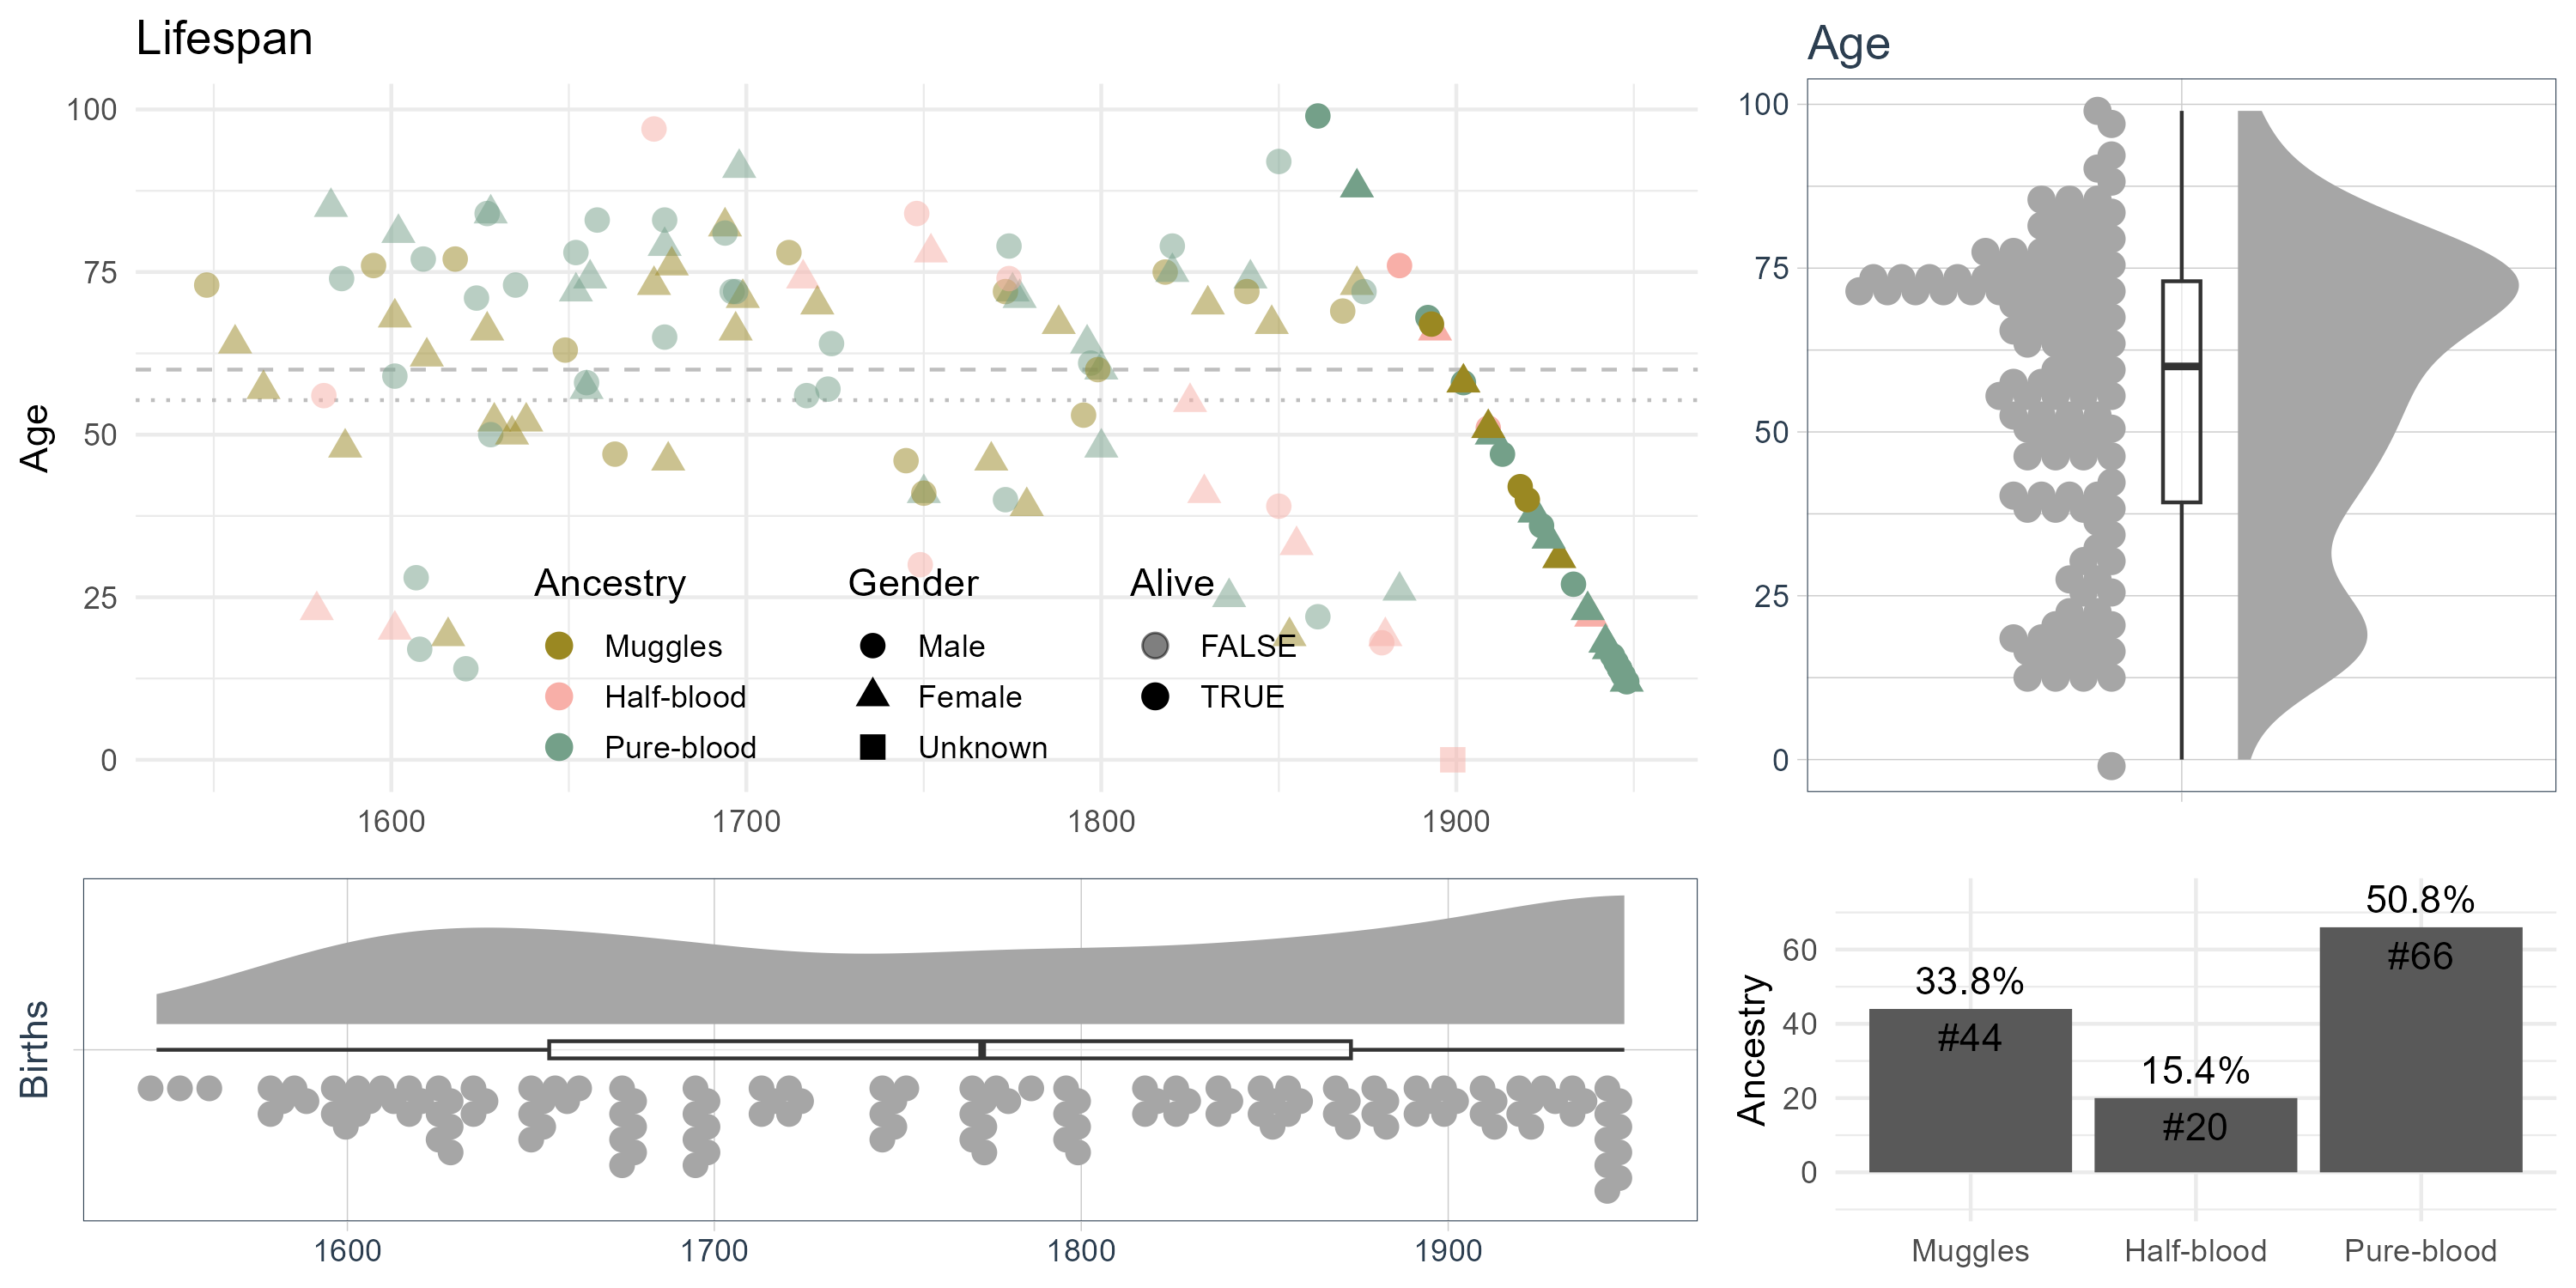
\includegraphics[width=\textwidth]{../rek-data-beers/R/figures/family_birth}
    \vspace{-18pt}
    \begin{itemize}
        \item Average woman lives 58.5 years (median 65, $n=50$)
        \item Average man lives 62.5 years (median 71, $n=49$)
        \item 1 centenarian, 4 people live to 90, 14 live to 80, 46 live to 70
    \end{itemize}
\end{frame}

\begin{frame}{Parental Age Trends \& Marital Age Gaps}
\note{
\begin{itemize}
\item Ice People women typically become mothers around 23.5 years, a choice influenced by prevalent dangers.
\item The curse dictates family size. One non-cursed child often stops family expansion, but a cursed birth may lead to larger families,
hoping the generation's \emph{curse quota} is filled.
\item Parental absence is a saga reality; a third of children grow up without a parent,
and it's not due to immaculate conceptions but the harsh reality of abandonment.
\item Yet, amidst these peculiarities, some aspects mirror our world. In 85\% of Ice People marriages, husbands are typically older by an average of three years — a trend not uncommon in our own society.

\end{itemize}
}    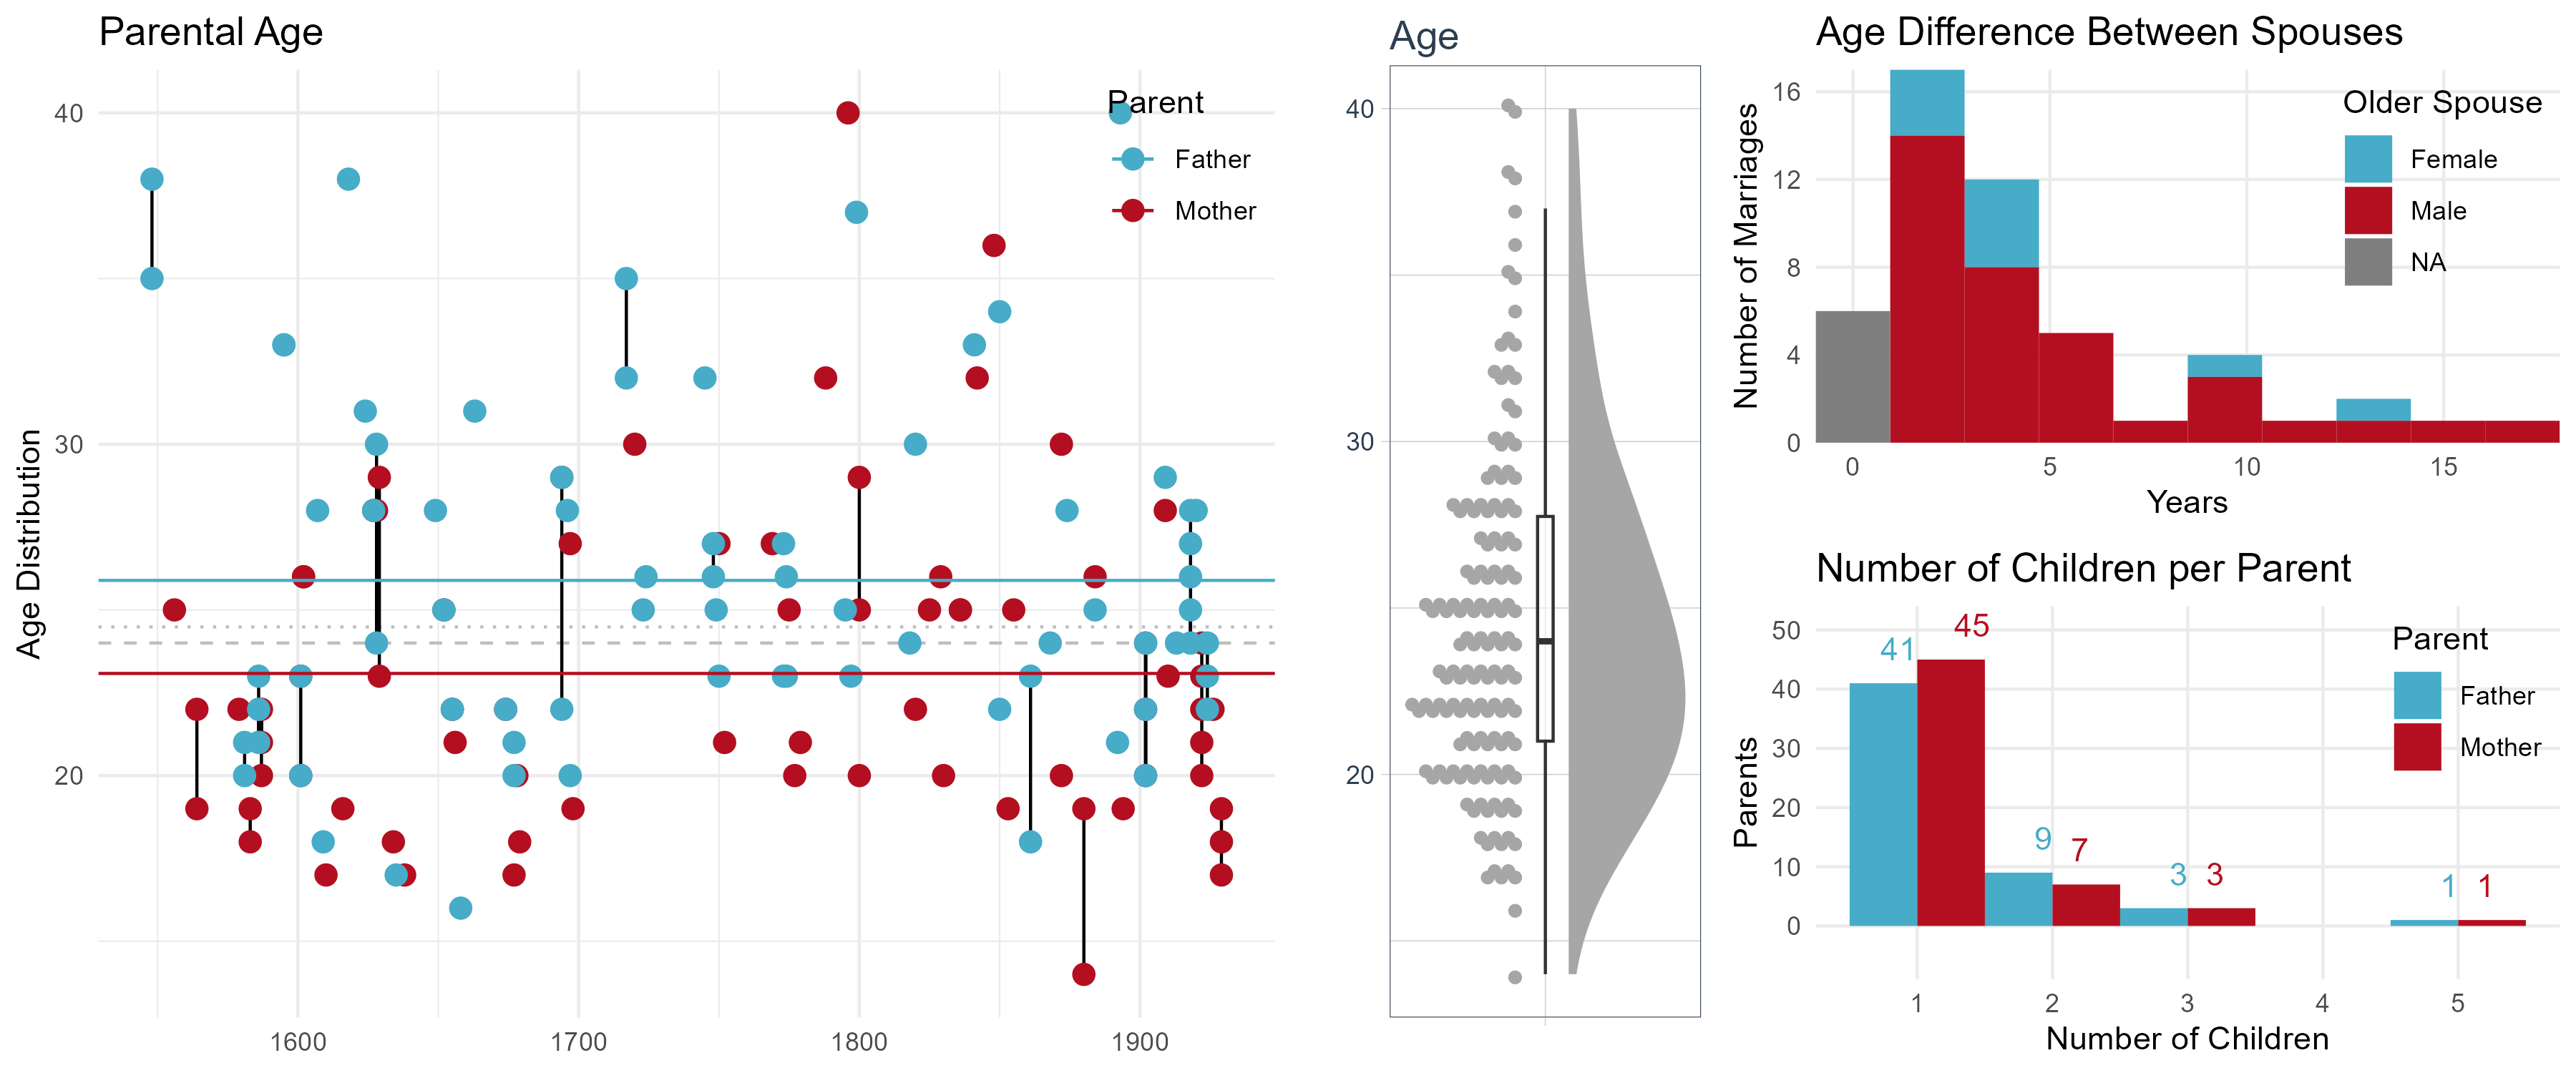
\includegraphics[width=\textwidth]{../rek-data-beers/R/figures/family_parent_age}
    \vspace{-18pt}
    \begin{itemize}
        \item 53 relationships described, 66 children born
        \item Average age of mother at childbirth is 23.5 years (fathers 26.0)
        \item 22 kids have either no father ($n=10$) or no mother ($n=12$)
        \item 85\% of marriages have an older husband, age difference generally 3 years (max 17 years)
    \end{itemize}
\end{frame}

\begin{frame}{Icelandic Naming Trends}
\note{\scriptsize
\begin{itemize}
\item In the 1980s, \emph{Ísfólkið} transcended literature, influencing Icelandic naming trends.
\item Names like \emph{Þula}, \emph{Yrja}, \emph{Heikir}, and \emph{Viljar} gained popularity post-publication, previously being unknown to Icelandic census.
\item There were significant surges: \emph{Sunna} increased 4-fold, \emph{Silja} doubled, and \emph{Saga} had a 5-fold jump.
\item Some name spikes, like \emph{Sölvi}, might be unrelated to the saga due to the character's malevolent nature.
\item However, names like \emph{Villimey} remained exclusive to the saga with no real-world adoptions.
\item Thanks to Yngvi Gautsson of \emph{Utopia Arctica} for the insightful data, helping clarify misconceptions from my earlier Reykjavík DataBeer Talk.
\end{itemize}
The saga's sway on Icelandic names emphasizes Margit's lasting cultural imprint.
}
    \centering
    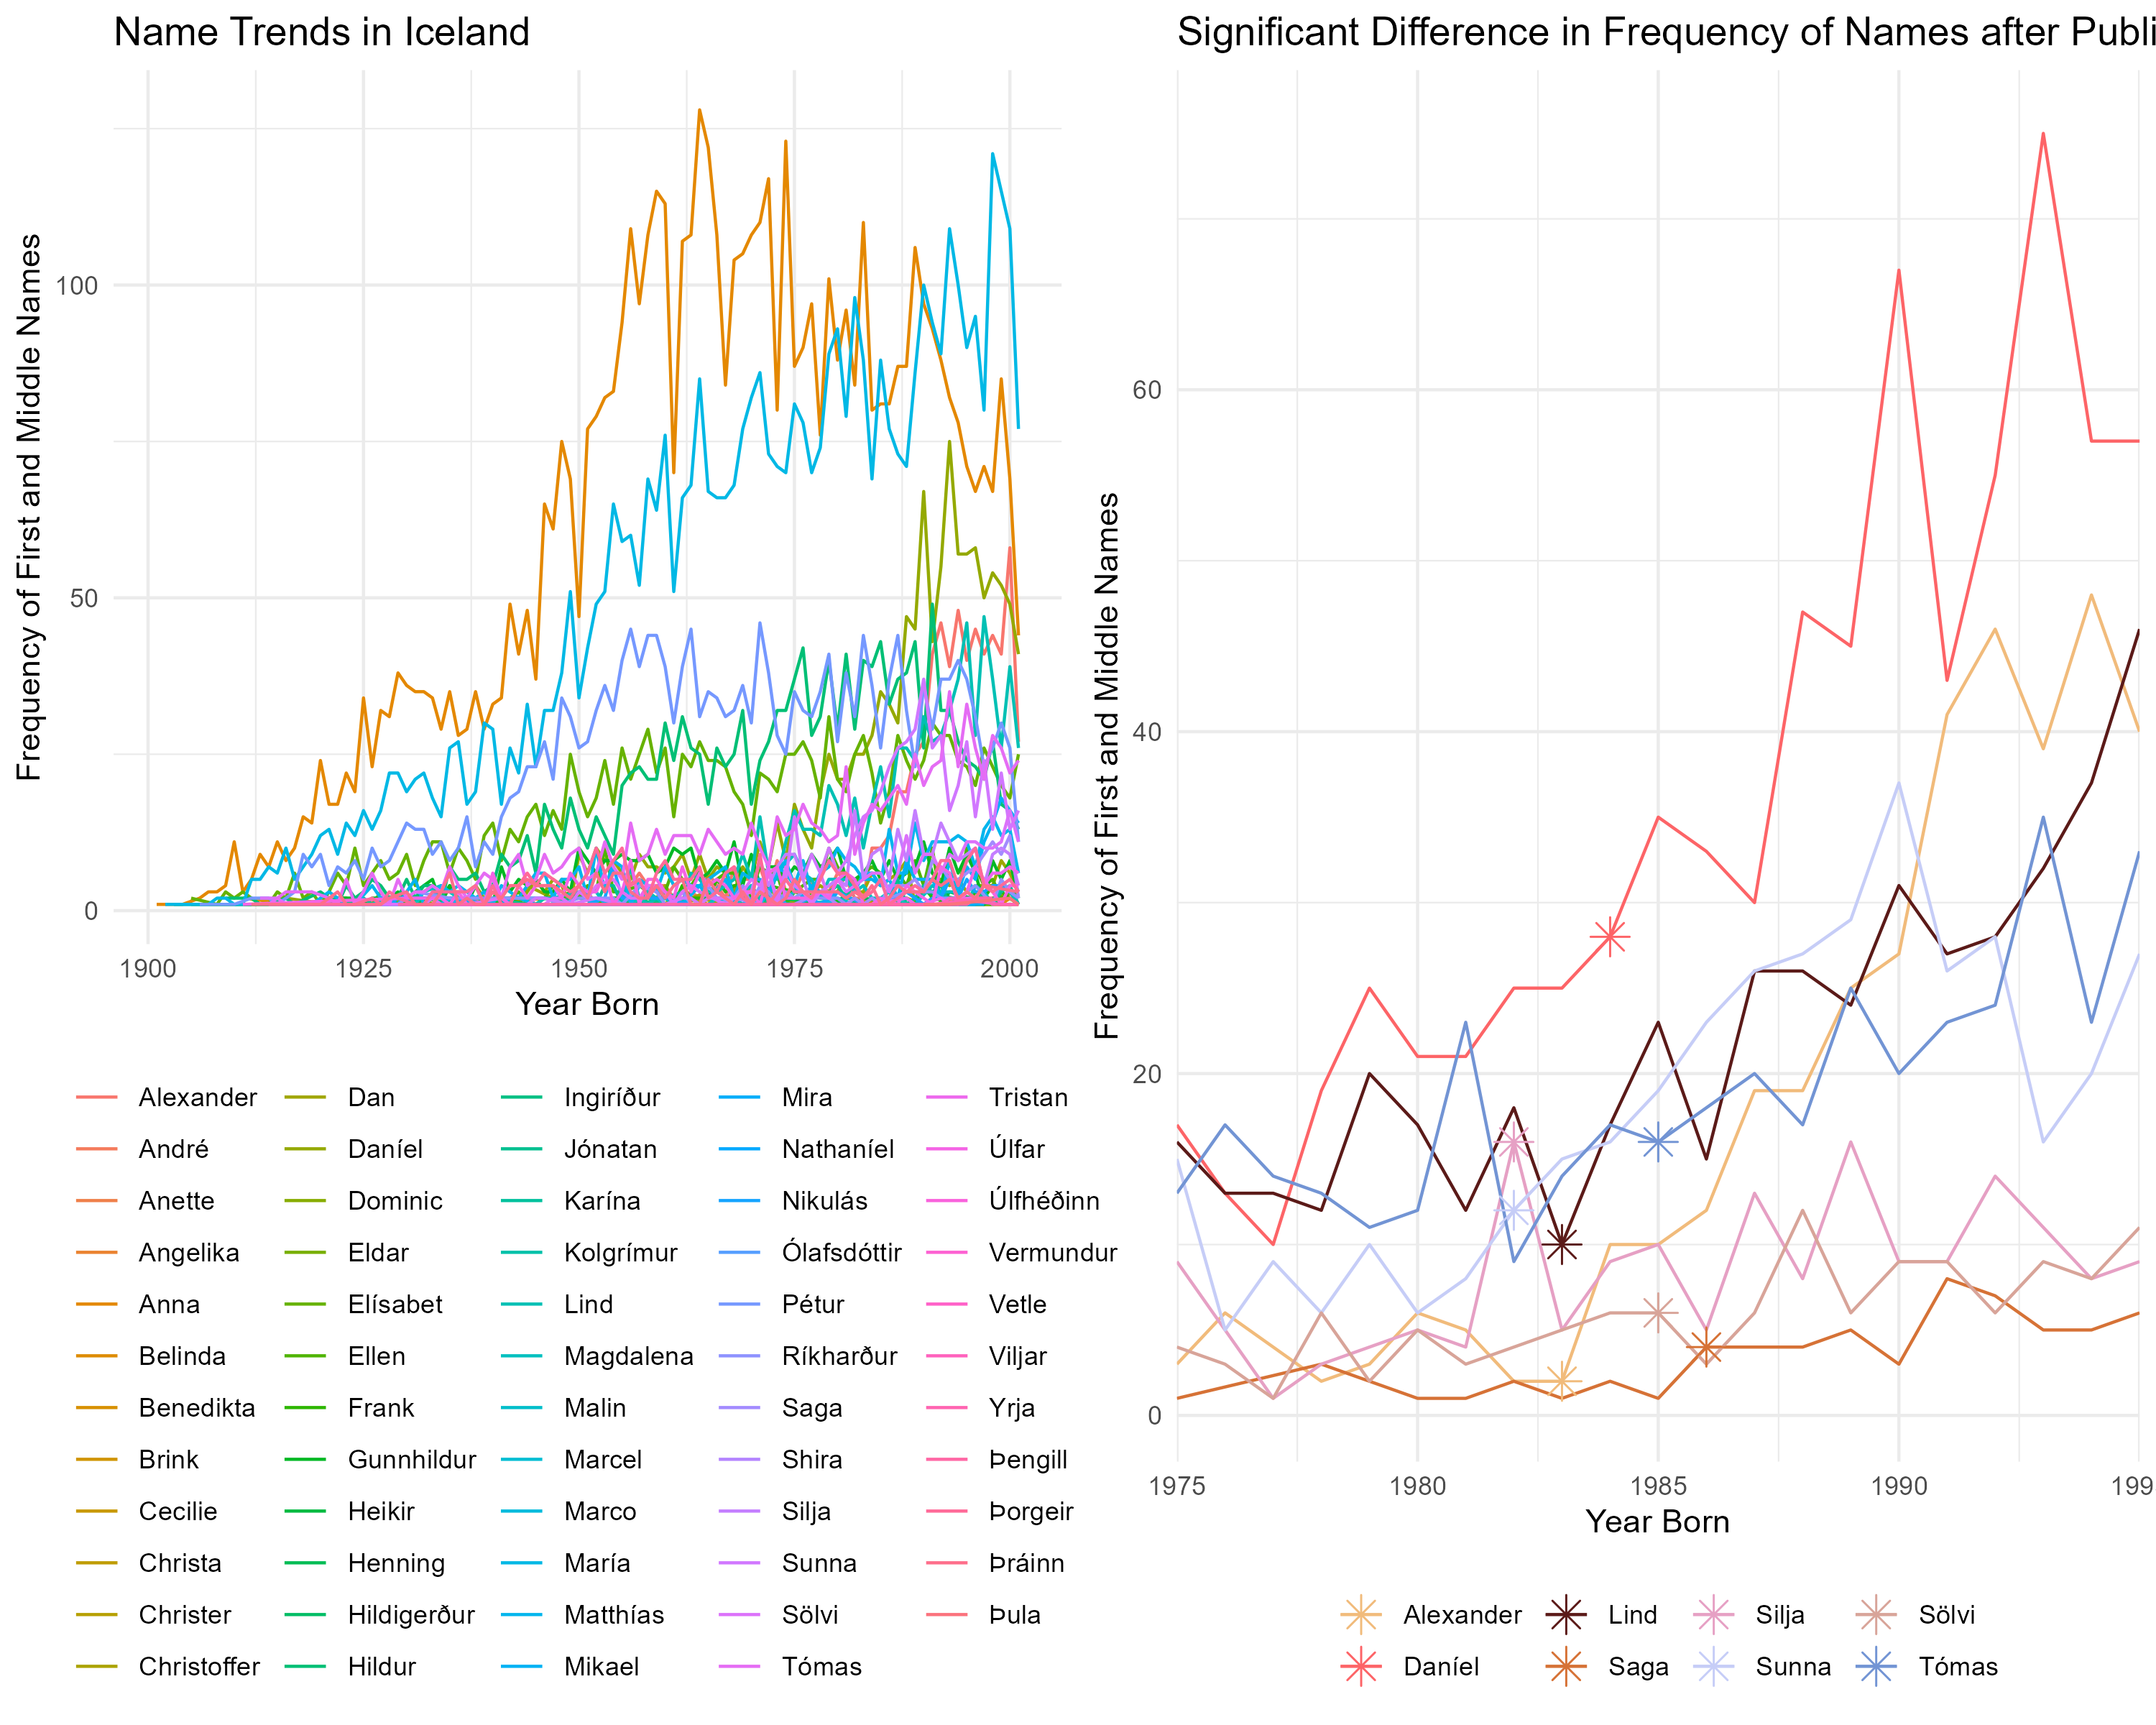
\includegraphics[width=\textwidth]{../rek-data-beers/R/figures/iceland_names.png}
    \vspace{-18pt}
    \begin{itemize}
        \item Protagonists' names \emph{Yrja}, \emph{Þula}, \emph{Heikir} and \emph{Viljar} first appear in the census
        a few years after Margit introduced them in her saga.
        \item Icelandic census data provided by Yngvi Gautsson of \emph{Utopia Arctica}
    \end{itemize}
\end{frame}
